%%%%%%%%%%%%%%%%%%%%%%%%%%%%%%%%%%%%%%%%%%%%%
\section{Visuals}
\label{sec:visuals}
%%%%%%%%%%%%%%%%%%%%%%%%%%%%%%%%%%%%%%%%%%%%%

Pangaea is composed of 3 primary visual components. Each component is
tailored to understanding systems at different granularities. The
first component is the time curve. The time curve plots a point for
each snapshot collected from a systems logs. The distance between each
point is the difference in their state as calculated in
Section~\ref{differentiation-algorithm}. The points are connected by a
curve which links them temporally, creating an approximate FSM from
the execution. Second likely data invariants, mined from the logs, are
plotted graphically. Points in the graph are logged variables collected
from all nodes present at runtime. Edges connecting the points are
invariants on their values. Finally Pangaea renders a ShiViz style
communication graph. The vertical lines of the graph correspond to
individual nodes. Edges between the vertical lines are messages sent
between the nodes. Together these visuals provide a comprehensive view
of the systems runtime behaviour.

To generate examples of our visualizations we instrumented and
executed a three node cluster of etcd~\cite{etcdraft}. Etcd is a
popular, and industrial scale raft implementation. Raft is a fault
tolerant concuss algorithm. Etcd raft implements a key value store
which allows users to issue put and get requests. For the sake of
example our visualization were taken from a run in which a client
issued 50 put requests, followed by 50 get requests.

\subsection{Time Curve}
\label{sec:time-curve}


Each point in the time curve correlates to a single snapshot.  Therein
each point is representative of the system as a whole.  A result of
calculating the differential of each snapshot, is that system states
which are similar to one another are clustered together, while
differing states are further apart.  This clustering allows users to
quickly associate similar states of their system. Each point is also
color coded based on their temporal ordering. The first snapshot is
colored bright red, and the final snapshot is dark brown. All
intermediate points are colored as an intermediate hue. By coloring
each of the points users can associate clustered state with a time in
the systems execution. The starting and end snapshots are significant
because they orient the users reasoning about their system. Starting
and end points are circled in blue to make them identifiable.

All points in the graph are connected by a single curve. The curve
begins at the starting point, ends at the end point, and connects all
points sequentially as they occur in logical time. The curve is color
coded identically with the points. It begins as bright red, and
transitions to dark brown. Where the curve intersects with a point
their colors match. The purpose of color coding the time curve is to
allow users to quickly associate a temporal relationship on
transitions between states. A legend which describes these encodings
is positioned in the top right of the graph.

Users interact with the curve by selecting an individual snapshot.
When selected concrete information about the snapshot is provided to
the user. First, the corresponding cut of the network from on which
the snapshot was taken is highlighted on the process communication
graph (see Section~\ref{sec:communication-graph}). Second the user is
presented with a table of variables and their values from the
snapshot. The table contains information about the node a variable was
resident on, the name of the variable, the variables type, and its
value. Additionally a table containing the vector clocks on each node
is rendered to help users identify the precise moment the snapshot was
taken. Concrete values allow users to reason precisely about the state
of the system. Users can investigate which variable assignment
correspond to clusters in the curve. In the cases of divergent or
unexpected clustering users can associate concrete state with the
behaviour of their system.

In Figure~\ref{fig:put-get-curve} the bright red cluster, and brown
cluster correspond to snapshots in which put, and get requests were
being serviced respectively. A single connection in the curve links the
red cluster to the brown cluster and denotes the transition from one
distinct functionality to the next. A small cluster containing the
initial snapshot is differentiated from the two main clusters. This
small cluster corresponds to a leader election triggered at the
beginning of the clusters execution.

\begin{figure}[h]
    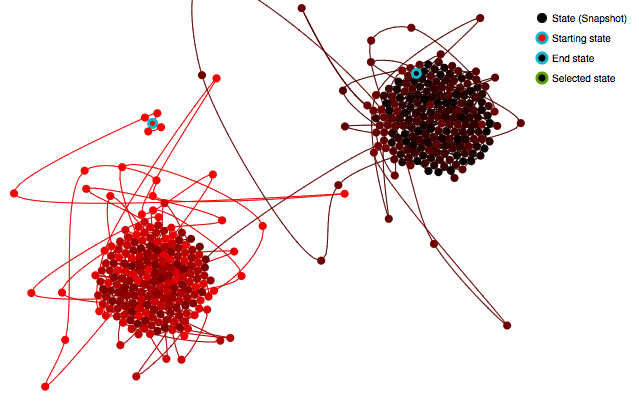
\includegraphics[width=\linewidth]{fig/put-get-curve}%
    \caption{Time curve generated from an etcd raft cluster processing 50 put requests, followed by 50 get requests.\label{fig:put-get-curve}}%
\end{figure}
    


\subsection{Invariant Graph}
\label{sec:invariant-graph}

The invariant graph is composed of points, corresponding to variables,
and edges, which are invariant relationships between the variables.
The invariants Pangaea renders are calculated by Dinv~\cite{dinv}.
Dinv reports invariants in the same format as Daikon~\cite{Ernst01}.
Figure~\ref{fig:dinv-output} is Dinv's invariant output from analyzing
etcd raft. These invariants can be difficult to comprehend for
developers unfamiliar with the format. Further the textual representation
obfuscates the transitive properties of the invariants, requiring the
user to reason about them.

Pangaea graphs the systems invariants to present them intuitively, in a
way which communicates the transitive nature of the invariants. We
implemented four invariant encodings for relationships which hold over
integers, and a subset of which hold over more general types.
Specifically a thin black line denotes equality, while a dashed black
line denotes inequality. Both of these relationships are valid on
arbitrary data so they are graphed for all types, such as strings,
booleans, and integers. Light blue triangular edges correspond to the
\emph{less than} relationship. Two corners of the triangle are attached
to the greater variable, while a single is attached to the lesser.
Similarly a light blue triangle with a black border represents the
\emph{greater than or equal too} relation. Users can select a
variable, and all transitive relations are highlighted in red. When a
variable is highlighted, and variables which do not have a transitive
relationship have their names removed from the graph, to increase
legibility.

Figure~\ref{fig:invariant-graph} is an invariant graph generated from
Dinv's invariant output in Figure~\ref{fig:dinv-output}.
Figure~\ref{fig:invariant-graph}A is the static representation of the
graph.  All variable names, and relationships are visible to the
user. Figure~\ref{fig:invariant-graph}B is the result of a user clicking
on the \emph{C-state} point.

\begin{figure}[h]
    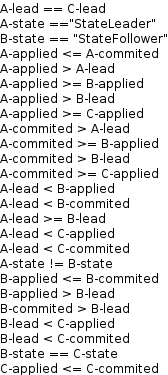
\includegraphics[width=0.5\linewidth]{fig/dinv-output}%
    \caption{Dinv's invariant output from analyzing etcd.\label{fig:dinv-output}}%
\end{figure}

\begin{figure}[h]
    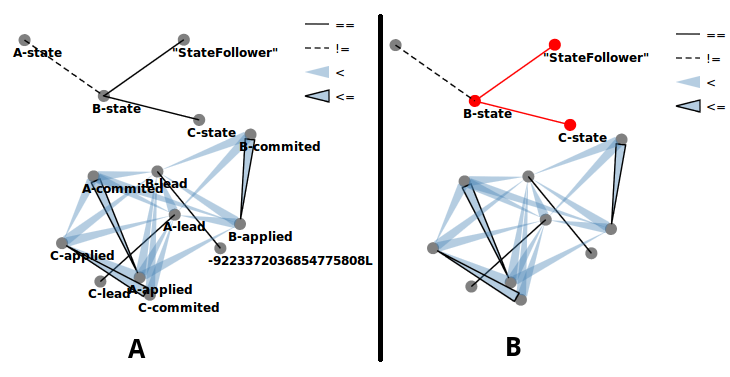
\includegraphics[width=\linewidth]{fig/invariant-graph}%
    \caption{Pangaea's invariant graph generated from Dinv's invariants in Figure~\ref{fig:dinv-output}.A) is a static rendering of the invariants. B) User selected invariants \label{fig:invariant-graph}}%
\end{figure}

\subsection{Communication Graph}
\label{sec:communication-graph}

The communication graph is a directed acyclic graph of node
communication. Vertical lines are unique to individual nodes, and are
assigned a unique color for legibility. At the top of each vertical
line is a square, denote the beginning of an execution, and the name
of the node which the line corresponds to. Circles on each nodes line
are logged events. A diagonal line between events on separate nodes is
a message sent from the node at the top of the diagonal, to the node
at the bottom of the diagonal. Pangaea communication graph is a
re-implementation of ShiViz's visualization~\cite{BeschastnikhWBE2016}.
The purpose of this visual is to help users reason the state of
snapshots. When a user selects a snapshot from the time curve graph
(Section~\ref{sec:time-curve}) gray boxes are added to each node line
at the logical time that the snapshot was taken. This feature allows
users to reason about how specific communication patterns have
influenced the state of their system.

Figure~\ref{fig:communication-graph} is the communication graph of an
etcd raft cluster. The sample is taken from the beginning of an
execution while an initial election takes place, and the nodes of the
cluster agree upon a configuration. The gray boxes correspond to the
logical time of the first snapshot of the system. This visual was
triggered after selecting the initial state from
Figure~\ref{fig:put-get-curve}.


\begin{figure}[h]
    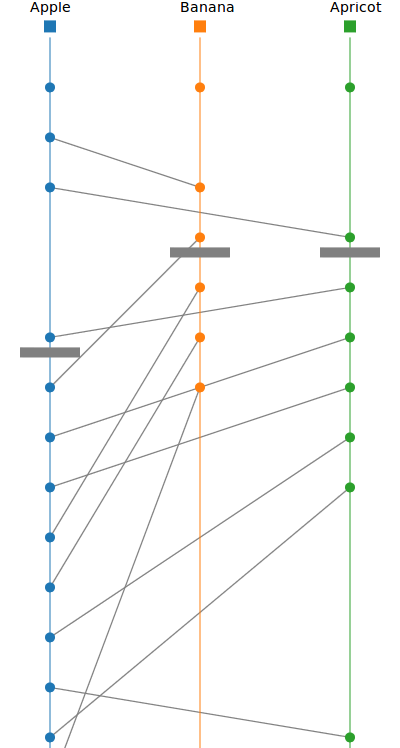
\includegraphics[width=\linewidth]{fig/communication-graph}%
    \caption{Communication graph of an etcd raft election; The first snapshot of the system was selected from the corresponding time curve.\label{fig:communication-graph}}%
\end{figure}


